\chapter{Addressing the Challenges of Radar-based Gesture Recognition} \label{chap:radar-challenges}

\begin{figure}
    \centering
    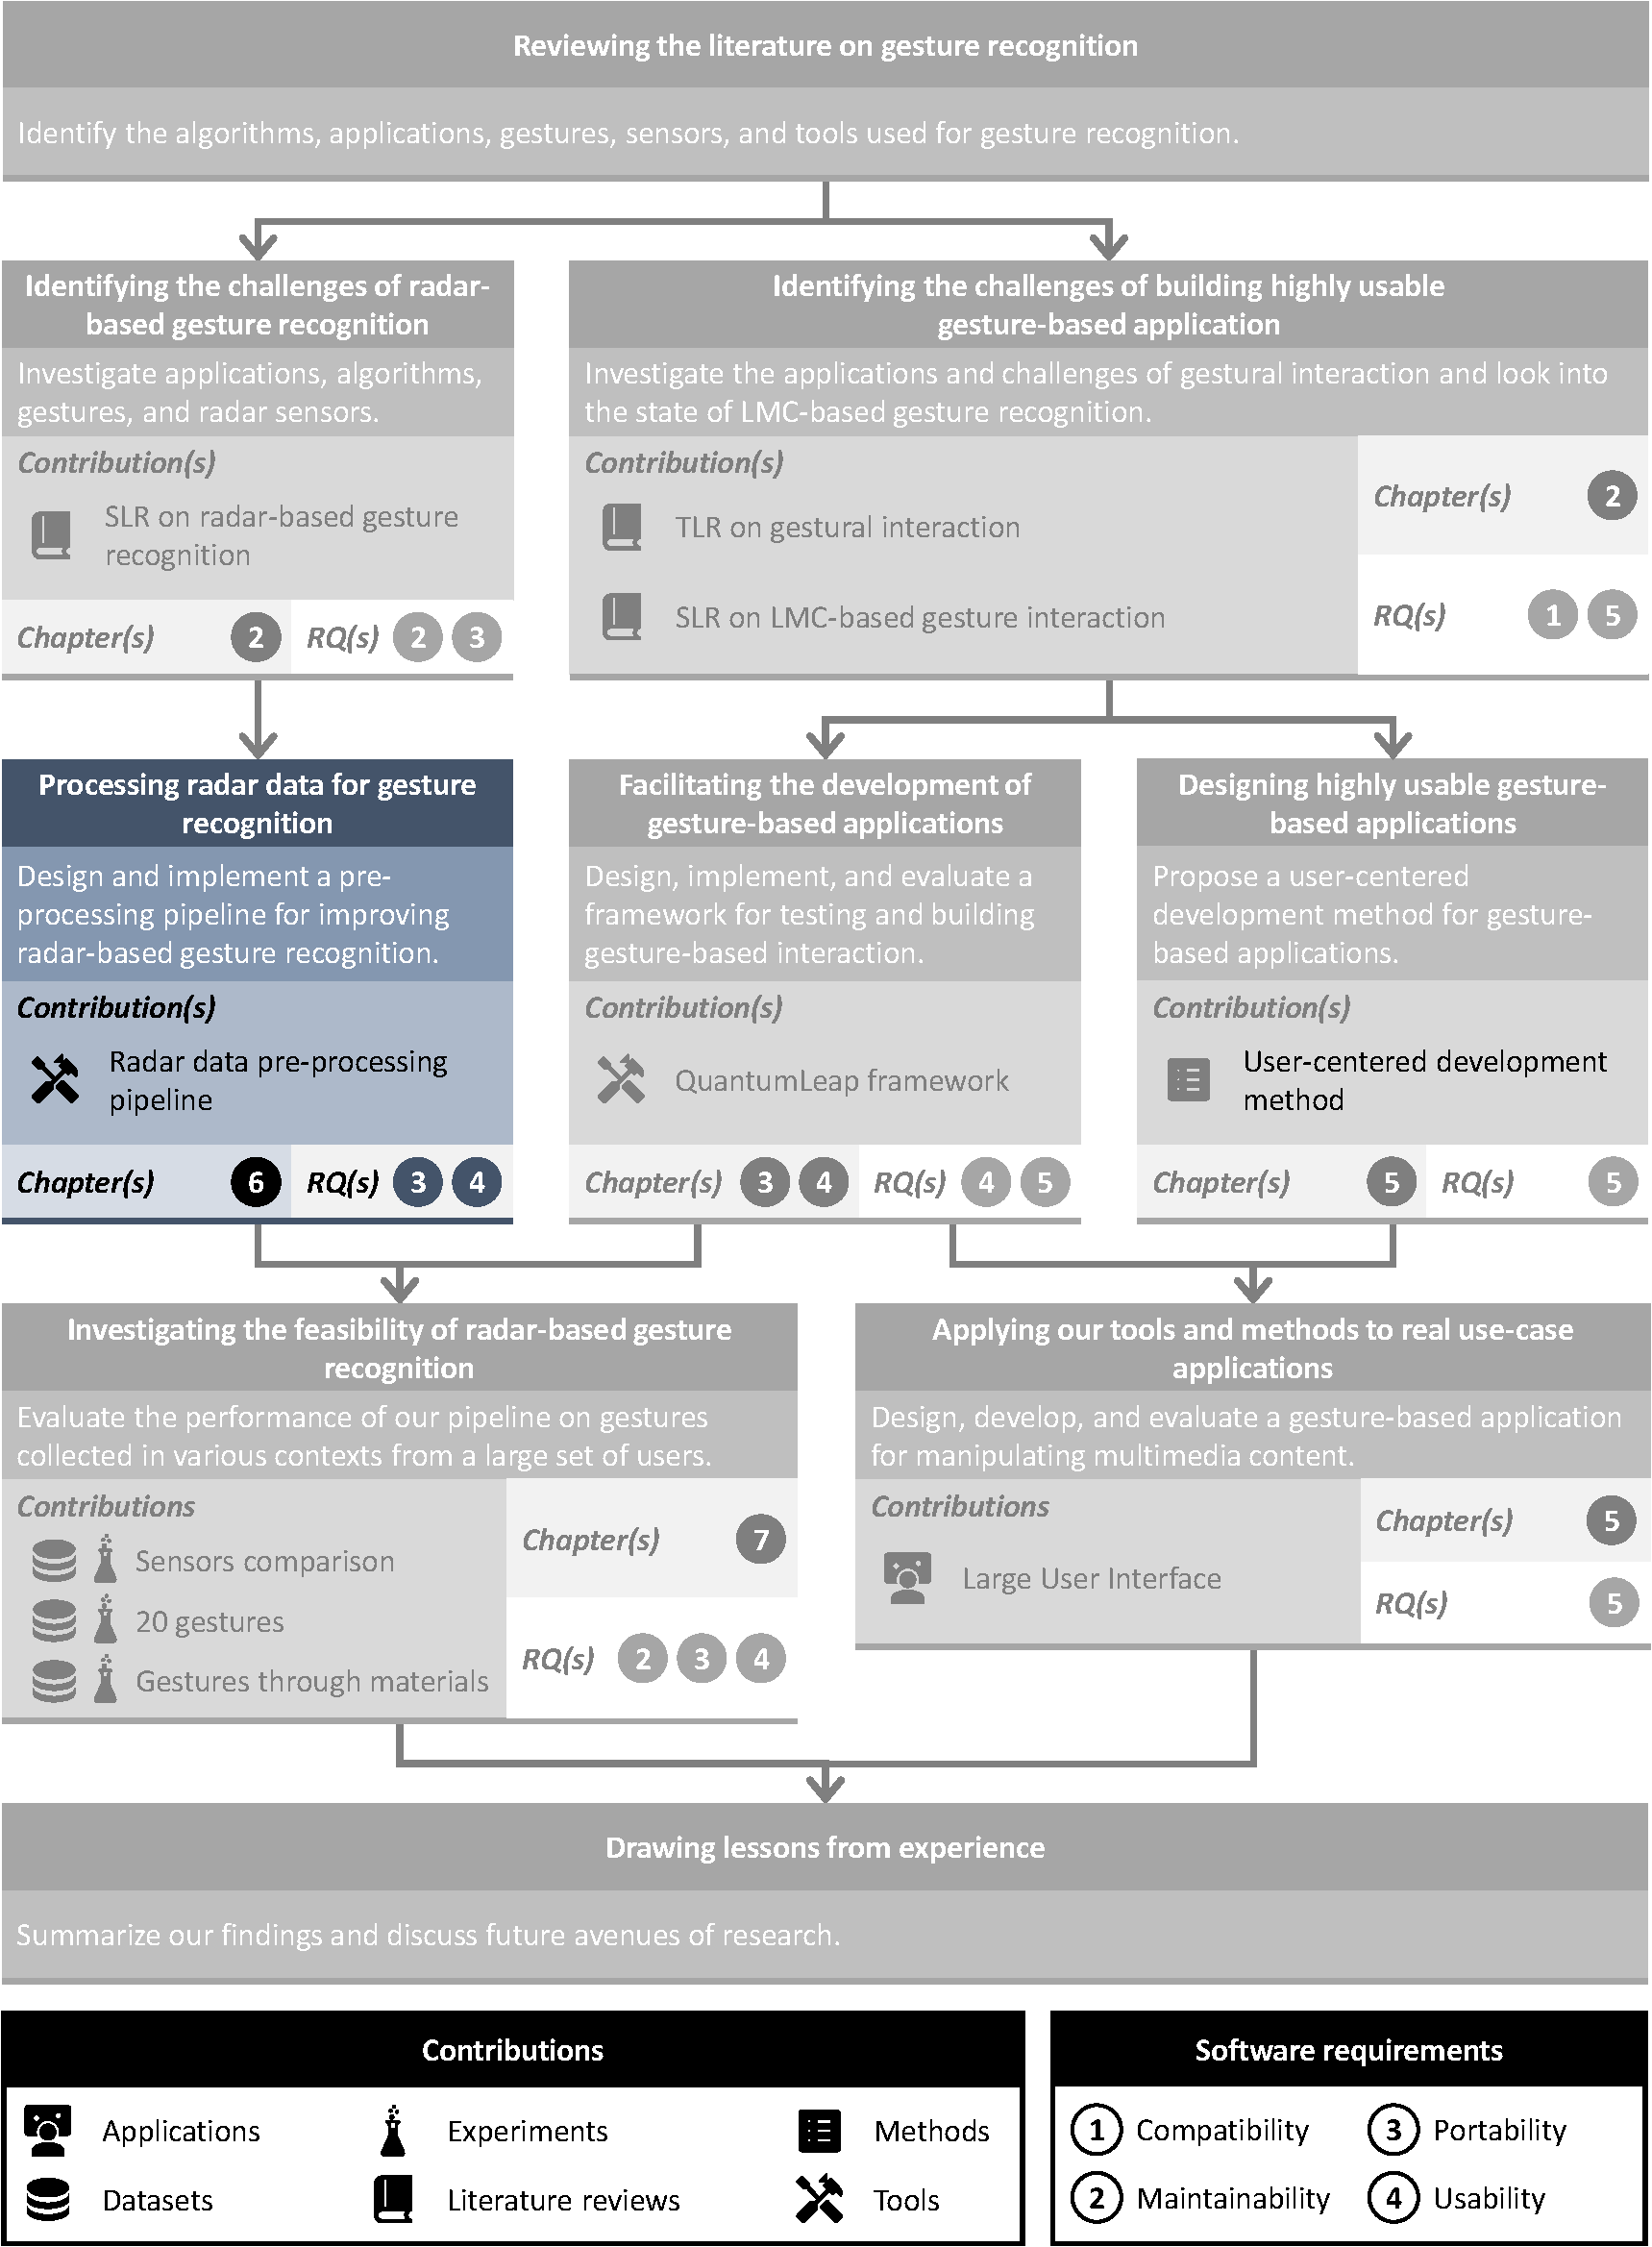
\includegraphics[width=\linewidth]{Figures/RadarChallenges/graphical-summary-radar-challenges.pdf}
    \vspace{-18pt}
    \caption{Main contributions of this chapter.}
    \label{fig:radar-challenges:graphical-summary}
\end{figure}

Radar sensors provide a unique alternative to other input devices (\eg vision-based sensors, IMUs) for gesture recognition. They combine a low sensitivity to lighting conditions, an ability to see through surfaces, and user privacy preservation with a small form factor and low power consumption. However, radar signals can be noisy, complex to analyze due to their high dimensionality~\cite{vanderMaaten:2009}, and usually do not transpose well from one radar to another.
%
Our SLR on radar-based gesture interaction (Section~\ref{sec:state_of_the_art:radar}) highlighted that most analyzed papers relied on deep learning techniques tailored to a specific radar and set of gestures. 
%
While these highly tailored solutions can achieve extremely accurate gesture recognition, they are difficult to adapt to other use cases (\eg sensors, gestures, and environments) and hinder the ability of end users to customize applications by defining their own set of gestures.
%
Consequently, few real applications have been developed, despite the remarkable potential of radar-based systems for gesture interaction.
%
In this context, this chapter addresses two of the five research questions defined in Section~\ref{sec:introduction:research:research-questions}: 
\begin{itemize}
    \item [RQ3] \textit{What types of gesture-based applications would benefit from radar sensors?}
    \item [RQ4] \textit{How can we foster collaboration between researchers and practitioners working on (radar) gesture recognition?}
\end{itemize}
To this end, we introduce a signal processing pipeline that employs full-wave electromagnetic modeling and inversion~\cite{Lambot:2004,Lambot:2014} and satisfies three properties to address the main challenges of radar-based gesture recognition: (1) radar system invariance, \ie the output signal is normalized to become independent from the radar, (2) background scene invariance, \ie the output signal is no longer affected by the background scene, and (3) one-shot calibration, \ie the system needs to be calibrated only once.

The rest of this chapter consists of four sections.
Section~\ref{sec:radar-challenges:mathematical-theory} first explains the mathematical theory for full-wave electromagnetic modeling and inversion.
Section~\ref{sec:radar-challenges:processing-strategy} then describes how we applied this theory in the six stages of our model-based approach for radar signal processing. 
Section~\ref{sec:radar-challenges:implementation} discusses the implementation of the pipeline and applies it to a simple application.
Finally, Section~\ref{sec:radar-challenges:conclusion} summarizes this section.

\paragraph{Publications.} This chapter is based on two papers published in the IUI 2022 conference proceedings (Best paper award)~\cite{Sluyters:2022:IUI}, and ACM TiiS journal~\cite{Sluyters:2023}.
% Not yet published:
% IEEE Sensors (2024?)
% IUI2024
% Book chapter

\paragraph{Resources.} Two demonstration videos of the prototype application built with the pipeline are accessible at \url{https://youtu.be/qmHcBuxU1ig} and \url{https://youtu.be/YlD-808gimw}.


%================================================================================%
\section{Mathematical Theory} \label{sec:radar-challenges:mathematical-theory}

%--------------------------------------------------------------------------------%
\subsection{Full-wave Radar Model} \label{sec:radar-challenges:mathematical-theory:radar-model}
% Explain in detail the Modelization
% Multiple reflections between antenna and medium

% Hypothesis: far-field: antennas reduced as a point source and receiver. 
% Lambot \etal~\cite{Lambot:2004}

The far-field full-wave radar equation \cite{Lambot:2004} assumes a homogeneous field distribution for the back-scattered field over the antenna aperture when the target is far enough from the antenna. The linear block diagram in \fig~\ref{fig:radar-challenges:ff-block-diagram} describes the antenna using four characteristic global reflection ($R$) and transmission ($T$) coefficients: $R_i(\omega)$, $T_i(\omega)$, $T_s(\omega)$, and $R_s(\omega)$, where $\omega$ is the angular frequency and $a(\omega)$ and $b(\omega)$ are the source and returned signals in the frequency domain, respectively. Wave propagation from the radar antenna to the target is described using the 3D multilayered media Green function, defined as the $x$-directed backscattered electric field for a unit-strength electric source, both located at the antenna phase center \cite{Chew:1990,Michalski:1990,Slob:2002,Lambot:2004}. This equivalent medium is used for our hand gesture application, as an analytical solution of Maxwell's equations exists, while for real hands a 3D numerical solution would be needed, but would be impractical in terms of computing resources and too complex to use.
% \begin{figure}[ht]
% \centering
% \begin{picture}(200,200)(0,0)
% \put(85,132){\framebox(30,16){\footnotesize $R_i(\omega)$}}
% \put(35,92){\framebox(30,16){\footnotesize $T_i(\omega)$}}
% \put(135,92){\framebox(30,16){\footnotesize $T_s(\omega)$}}
% \put(85,52){\framebox(30,16){\footnotesize $R_s(\omega)$}}
% \put(85,12){\framebox(30,16){\footnotesize $G_{xx}(\omega)$}} \put(50,60){\circle{6}}
% \put(150,140){\circle{6}} \put(50,180){\vector(0,-1){72}} \put(50,92){\vector(0,-1){29}}
% \put(50,57){\line(0,-1){37}} \put(50,20){\vector(1,0){35}} \put(50,140){\vector(1,0){35}}
% \put(85,60){\vector(-1,0){32}} \put(115,140){\vector(1,0){32}} \put(150,60){\vector(-1,0){35}}
% \put(150,20){\vector(0,1){72}} \put(150,108){\vector(0,1){29}} \put(150,143){\vector(0,1){37}}
% \put(115,20){\line(1,0){35}} \put(57,55){\tiny +} \put(51,68){\tiny +} \put(145,129){\tiny +}
% \put(138,142){\tiny +} \put(42,185){\footnotesize $a(\omega)$} \put(142,185){\footnotesize
% $b(\omega)$} \put(90,185){\footnotesize Radar} \put(84,98){\footnotesize Antenna}
% \put(60,0){\footnotesize Multilayered medium}
% \end{picture}
% \caption{Equivalent linear block diagram of the radar-antenna-medium to which corresponds the far-field radar equation \cite{Lambot:2004}.} \label{fig:radar-challenges:ff-block-diagram}
% \end{figure}
The equivalent linear block diagram shown in \fig~\ref{fig:radar-challenges:ff-block-diagram} is solved as follows:
\begin{equation}\label{eq:radar-challenges:sff3}
b(\omega) = a(\omega) R_{i}(\omega) + \frac{a(\omega) T_{i}(\omega) G_{xx}(\omega)}{1- R_{s}(\omega) G_{xx}(\omega)} T_{s}(\omega)
\end{equation}
Defining the ratio $S(\omega) = b(\omega)/a(\omega)$, like the so-called $S_{11}$ quantity measured by a Vector Network Analyzer (VNA), and the product $T(\omega) = T_{i}(\omega)T_{s}(\omega)$, Eq.~(\ref{eq:radar-challenges:sff3}) becomes~\cite{Lambot:2004}:
\begin{equation}\label{eq:radar-challenges:sff4}
S(\omega) = R_{i}(\omega) + \frac{T(\omega) G_{xx}(\omega)}{1- R_{s}(\omega) G_{xx}(\omega)}
\end{equation}

For a pulse radar, the quantity $s(t)$ is measured, with $t$ being time, and $b(\omega)$ is obtained using the Fourier transform:
\begin{equation}
\label{eq:radar-challenges:fft}
b(\omega)=\text{$\cal{F}$}\left\{
s(t)
\right\}=\int_{-\infty}^{\infty}s(t)e^{-2\pi j t \omega}dt
\end{equation}

Then, defining $H_i(\omega)=a(\omega) R_{i}(\omega)$, $H(\omega) = a(\omega) T(\omega)$ and $H_s(\omega) = R_{s}(\omega)$, Eq.~(\ref{eq:radar-challenges:sff3}) becomes:
\begin{equation}\label{eq:radar-challenges:sff5}
\text{$\cal{F}$}\left\{
s(t)
\right\} = H_{i}(\omega) + \frac{ H(\omega) G_{xx}(\omega)}{1- H_{s}(\omega) G_{xx}(\omega)}
\end{equation}
Whether the radar provides the ratio $b(\omega)/a(\omega)$ or the signal $b(\omega)$, the radar-antenna system is fully described by only three independent functions.
$R_i(\omega)$ or $H_i(\omega)$ corresponds to a free-space measurement, for which $G_{xx}(\omega)$ = 0, while $R_{s}(\omega)$ is responsible for the multiple reflections between the antenna and the target medium. Eq.~(\ref{eq:radar-challenges:sff4}) is analytically inverted to derive Green's function from the measurements, thereby filtering out the effects of the antenna and resulting in a normalized quantity that is independent of the radar in a given frequency range:
\begin{equation}\label{eq:radar-challenges:sff6}
G_{xx}(\omega) = \frac{S(\omega) -  R_{i}(\omega)}{T(\omega) + S(\omega)R_{s}(\omega) - R_{i}(\omega)R_{s}(\omega)}
\end{equation}

A practical application of the far-field radar equation is to improve radar imaging, \eg for landmine detection~\cite{Lopera:2007}.

\begin{figure}[t]
\centering
\begin{picture}(200,132)(0,0)
%132 ->96
\put(85,96){\framebox(30,16){\footnotesize $R_i(\omega)$}}
\put(35,68){\framebox(30,16){\footnotesize $T_i(\omega)$}}
\put(135,68){\framebox(30,16){\footnotesize $T_s(\omega)$}}
\put(85,40){\framebox(30,16){\footnotesize $R_s(\omega)$}}
\put(85,12){\framebox(30,16){\footnotesize $G_{xx}(\omega)$}} 

\put(50,48){\circle{6}}
\put(150,104){\circle{6}} 
\put(50,124){\vector(0,-1){40}} %180->132
\put(50,68){\vector(0,-1){17}}
\put(50,45){\line(0,-1){25}} 
\put(50,20){\vector(1,0){35}} 
\put(50,104){\vector(1,0){35}}
\put(85,48){\vector(-1,0){32}} 
\put(115,104){\vector(1,0){32}} 
\put(150,48){\vector(-1,0){35}}
\put(150,20){\vector(0,1){48}} 
\put(150,84){\vector(0,1){17}} 
\put(150,107){\vector(0,1){17}}
\put(115,20){\line(1,0){35}} 
\put(57,43){\tiny +} 
\put(51,57){\tiny +} 
\put(145,94){\tiny +}
\put(138,106){\tiny +} 
\put(42,129){\footnotesize $a(\omega)$} 
\put(142,129){\footnotesize
$b(\omega)$} \put(90,129){\footnotesize Radar} 
\put(84,74){\footnotesize Antenna}
\put(65,0){\footnotesize Multilayered medium}
\end{picture}
\caption{Equivalent linear block diagram of the radar-antenna-medium corresponding to the far-field radar equation \cite{Lambot:2004}.} \label{fig:radar-challenges:ff-block-diagram}
\end{figure}

%--------------------------------------------------------------------------------%
\subsection{Determination of the Radar-antenna Characteristic Functions} \label{sec:radar-challenges:mathematical-theory:characteristic-functions}
The radar characteristic functions $R_i(\omega)$, $T(\omega)$ and $R_s(\omega)$ (or $H_i(\omega)$, $H(\omega)$ and $H_s(\omega)$) can be determined by solving a system of equations (\ref{eq:radar-challenges:sff4}) containing at least three different model configurations (denoted $k$). For our practice, the antenna is positioned at varying distances from a metal sheet, representing an infinite Perfect Electric Conductor (PEC). Knowing the properties of the medium, Green's functions are computed and the corresponding $S_{k}(\omega)$ are measured. The system of equations can be expressed in a linear form by reformulating Eq.~(\ref{eq:radar-challenges:sff4}) assuming frequency dependence $\omega$:
\begin{equation}\label{Art5S11r}
 S_{k} = R_i + S_{k}G_{xx,k}R_s + G_{xx,k} \left( T-R_iR_s \right)
\end{equation}
Hence, the resulting linear system of equations can be written in matrix form as:
\begin{equation}
\mathbf{b}=\mathbf{A}\mathbf{x}
\end{equation}
where
\begin{equation}
\mathbf{b}=
\begin{bmatrix}
 S_{1} \\
 \vdots \\
 S_{k} \\
 \vdots \\
 S_{n} \\
\end{bmatrix},
\mathbf{A}=
\begin{bmatrix}
 1 & S_{1}G_{xx,1} & G_{xx,1} \\
 \vdots & \vdots & \vdots \\
 1 & S_{k}G_{xx,k} & G_{xx,k} \\
 \vdots & \vdots & \vdots\\
  1 & S_{n}G_{xx,n} & G_{xx,n} \\
\end{bmatrix},
\mathbf{x}=
\begin{bmatrix}
 R_i \\
 R_s \\
 T-R_iR_s \\
\end{bmatrix}
\end{equation}

% \begin{equation}
% \mathbf{b}=
% \begin{bmatrix}
%  S_{1} \\
%  \vdots \\
%  S_{k} \\
%  \vdots \\
%  S_{n} \\
% \end{bmatrix}
% \end{equation}

% \begin{equation}
% \mathbf{A} =
% \begin{bmatrix}
%  1 & S_{1}G_{xx,1} & G_{xx,1} \\
%  \vdots & \vdots & \vdots \\
%  1 & S_{k}G_{xx,k} & G_{xx,k} \\
%  \vdots & \vdots & \vdots\\
%   1 & S_{n}G_{xx,n} & G_{xx,n} \\
% \end{bmatrix}
% \end{equation}

% \begin{equation}
% \mathbf{x}=
% \begin{bmatrix}
%  R_i \\
%  R_s \\
%  T-R_iR_s \\
% \end{bmatrix}
% \end{equation}

The vector of unknowns is then determined using the least squares approach:
\begin{equation}
\mathbf{x}=\left(\mathbf{A}^{\text{H}}\mathbf{A}\right)^{-1}\mathbf{A}^{\text{H}}\mathbf{b}
\end{equation}
where symbol H denotes the Hermitian or conjugate transpose
($\mathbf{A}^{\text{H}}\equiv\overline{\mathbf{A}^{T}}$). In order for the Green's function model to apply, which assumes infinite layers, the metal sheet should be larger than five times the maximum wavelength, depending on the antenna radiation pattern. For smaller sizes, the edge effects can affect the results.

%--------------------------------------------------------------------------------%
\subsection{Full-Wave Signal Inversion} \label{sec:radar-challenges:inversion}
% Inversion process
% LUT to speed up computations
Full-wave inversion can be used to determine the properties of the layered medium, by minimizing an objective function formulated in the least squares sense, expressed as:
\begin{equation}\label{OF}
\phi(\mathbf{b})=
\left|\mathbf{G^*_{xx}}-\mathbf{G_{xx}}\right|^T\mathbf{C}^{-1}
\left|\mathbf{G^*_{xx}}-\mathbf{G_{xx}}\right|
\end{equation}
where $\mathbf{G^*_{xx}}=G_{xx}(\omega)$ and $\mathbf{G_{xx}}=G_{xx}(\omega,\mathbf{b})$ are the vectors containing the measured and simulated radar signals, respectively. The vector $\mathbf{b}=[\varepsilon_n, \sigma_n, h_n]$ with $n=1,...,N$ contains the unknowns, while $\mathbf{C}$ is the measurement error covariance matrix. The discrepancy between observed and modeled data is expressed by the amplitude of the errors in the complex plane, where the radar data vectors are arranged by frequency since the radar data are complex-valued. To focus on a particular range window, containing for example the medium surface only \cite{Lambot:2006}, inversion is performed in the time domain. The reflections occurring after the reflection of interest are thereby disregarded and the inverse model configuration can be simplified, e.g., reducing it to a half-space medium. To convert the frequency domain data into the time domain, the Inverse Fast Fourier Transform (IFFT) is applied:
\begin{equation}
\label{eq:radar-challenges:ifft}
g_{xx}(t)=\text{$\cal{F}$}^{-1}\left\{
G_{xx}(\omega)
\right\}=\int_{-\infty}^{\infty}G_{xx}(\omega)e^{2\pi j \omega
t}d\omega
\end{equation}
Then, a maximum time $t_{max}$ can be set to focus on the initial reflectors of interest, such as the surface reflection (\fig~\ref{fig:radar-challenges:tw}). The objective function becomes:
\begin{equation}\label{eq:radar-challenges:OFTD}
\phi(\mathbf{b})=
\left(\mathbf{g_{xx}^{*}}-\mathbf{g_{xx}}\right)^T\mathbf{C}^{-1}
\left(\mathbf{g_{xx}^{*}}-\mathbf{g_{xx}}\right)
\end{equation}
where
\begin{equation}\label{eq:radar-challenges:tmax}
\mathbf{g_{xx}^{*}}=\left.g_{xx}^{\uparrow*}(t)\right|_{0}^{t_{max}}
\quad\text{and}\quad
\mathbf{g_{xx}}=\left.g_{xx}(t,\mathbf{b})\right|_{0}^{t_{max}}
\end{equation}
are the vectors containing, respectively, the observed and simulated
time-domain windowed Green functions. Depending on the number of unknowns to estimate and the information available from the radar data, the topography of the objective function to be optimized can be quite complex, and in some cases, the inverse problem can be ill-posed. When dealing with one or two unknowns, local optimization using a method such as the Levenberg-Marquardt Algorithm (LMA)~\cite{Marquardt:1963} or a Look-Up Table (LUT) approach, which calculates the objective function across the entire parameter space, is reliable and efficient. However, for more complex problems, global optimization is usually required. 

\begin{figure}[t]
\noindent \centering

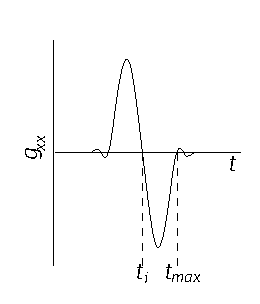
\includegraphics[width=0.4\columnwidth,trim={0 0 0 0.6cm},clip]{Figures/RadarChallenges/Theory/twr.eps}
\vspace{-4pt}
\caption{Sketch of the radar signal in the time domain, $g_{xx}$($t$), with antenna effects removed. The time window for the inversion, denoted as $t_{max}$, is chosen to focus, as an example, on the surface reflection. $t_i$ denotes the approximate time corresponding to the surface interface for the Green's function.} 
\label{fig:radar-challenges:tw}
\vspace{-12pt}
\end{figure}


%================================================================================%
\section{Radar Data Processing Strategy} \label{sec:radar-challenges:processing-strategy}

\begin{figure*}[t]
\centering
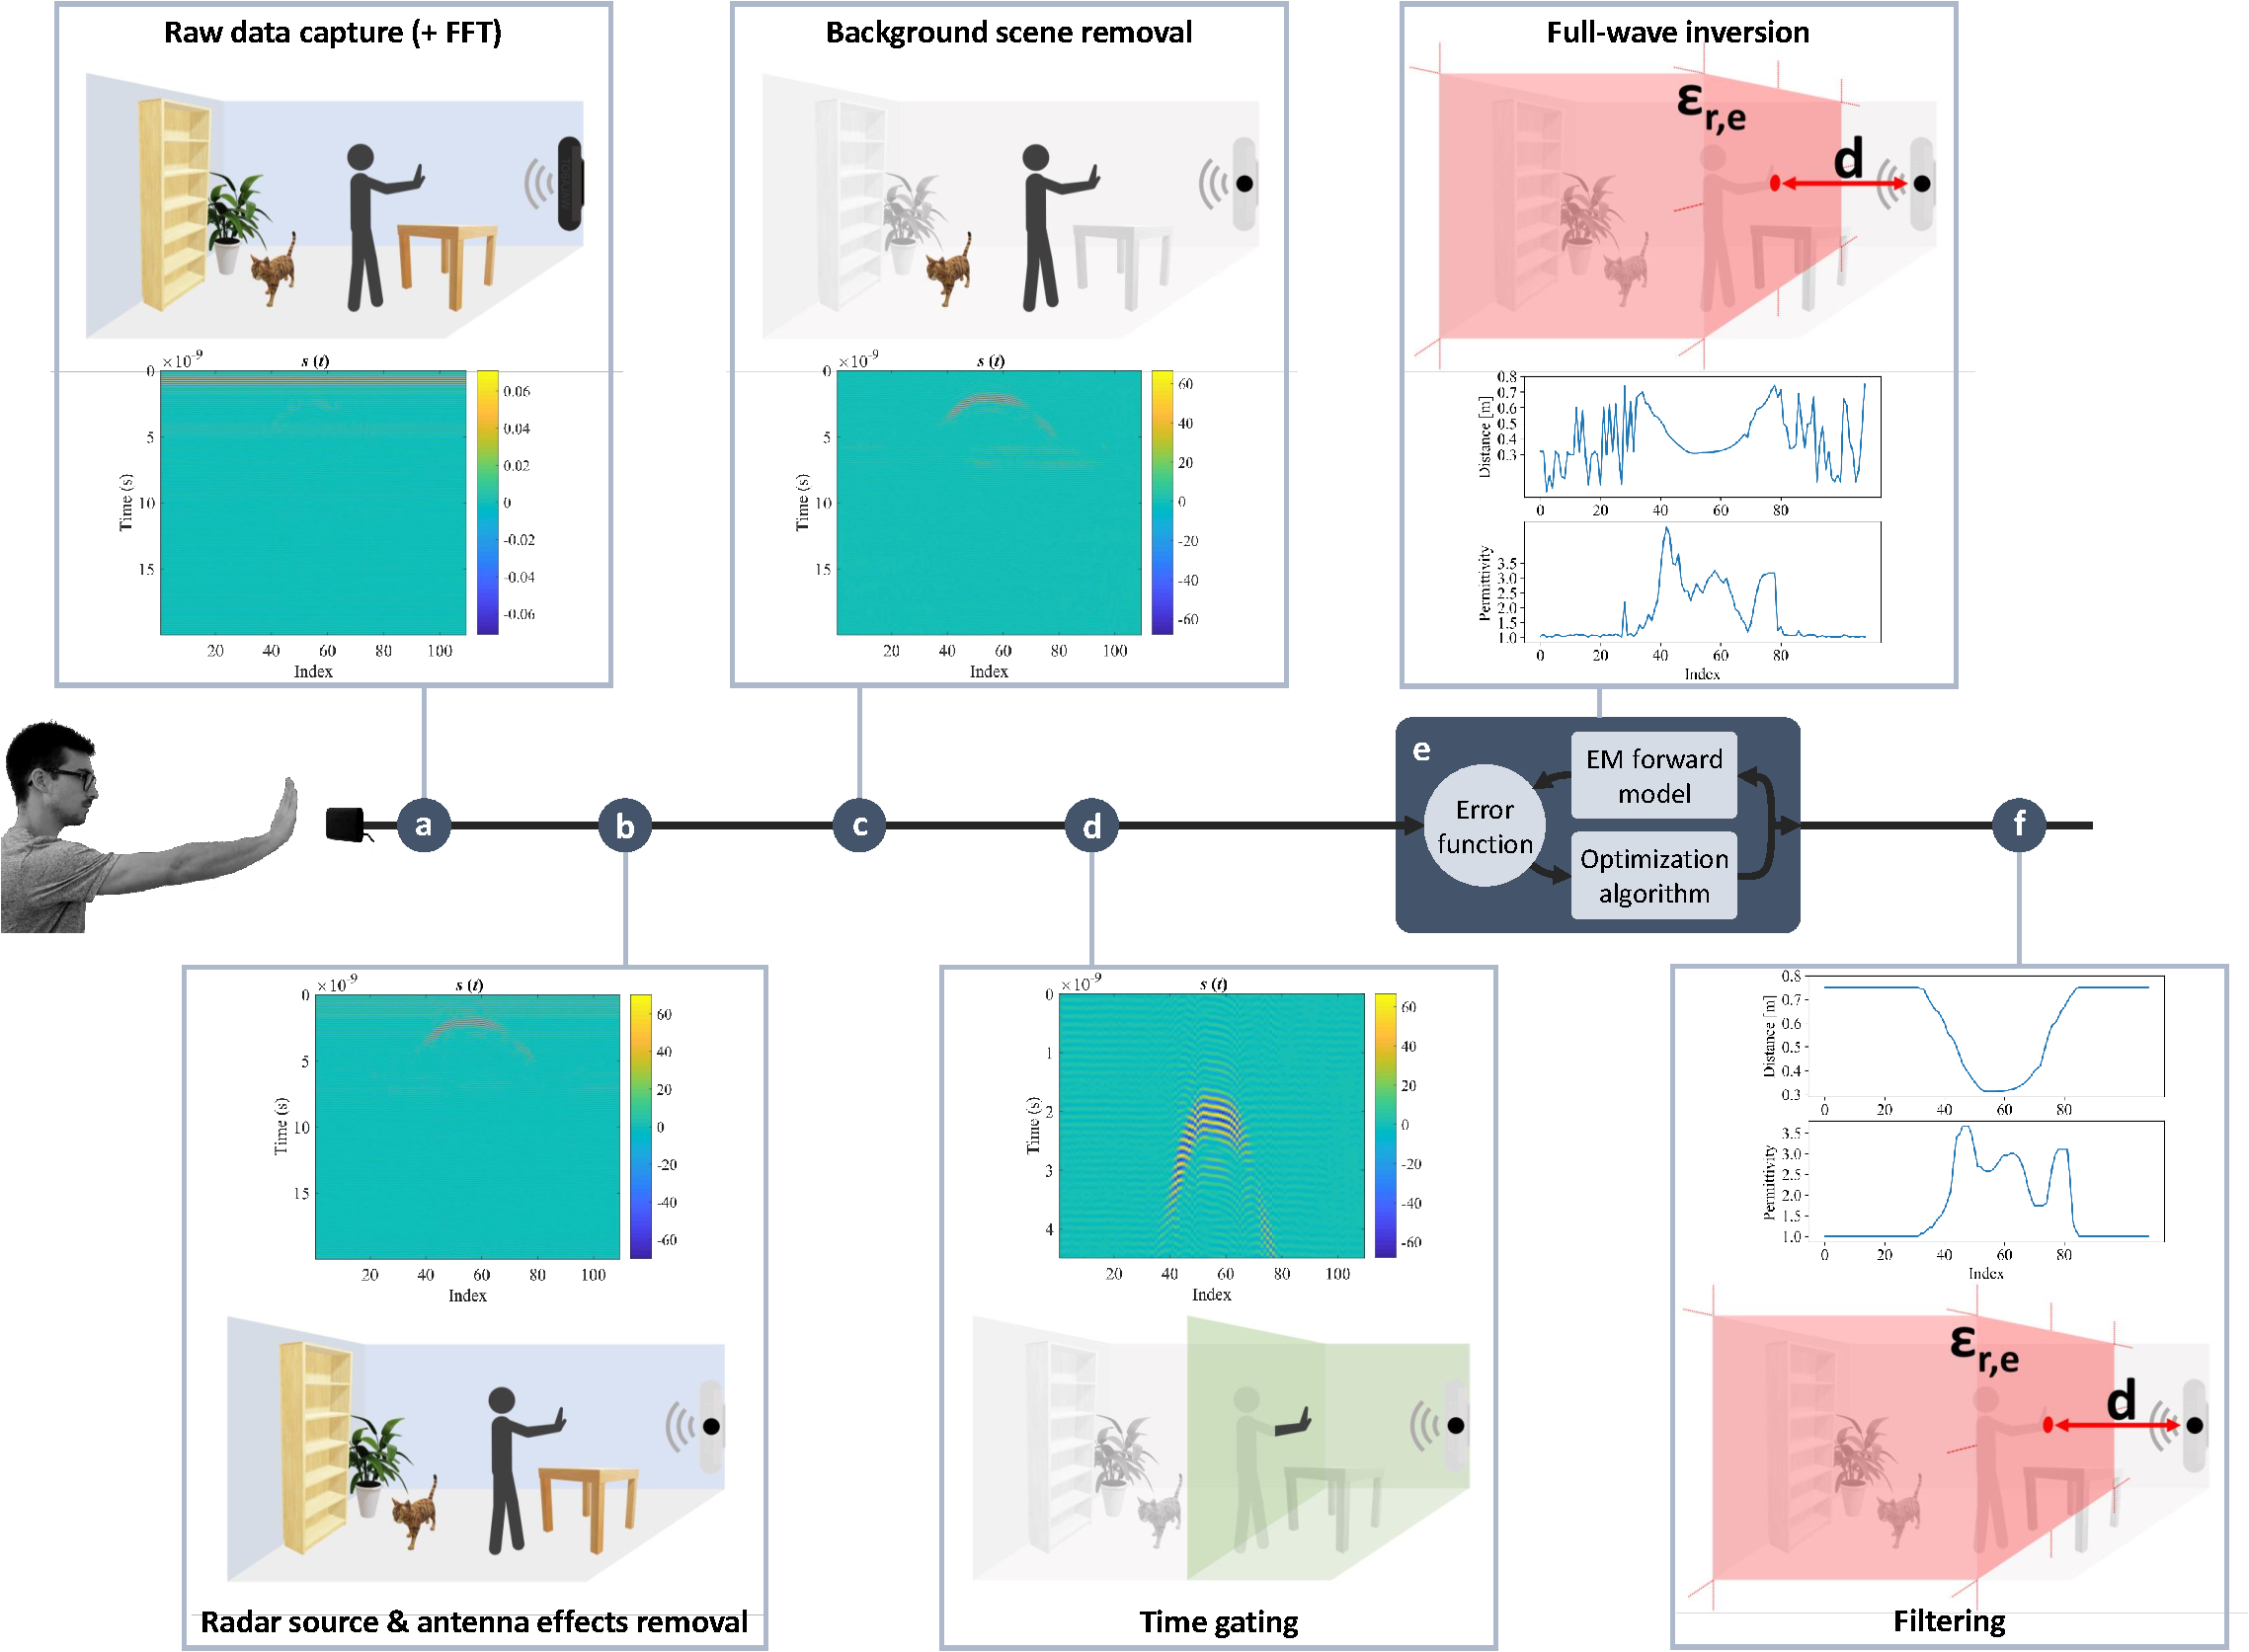
\includegraphics[width=\linewidth,trim={0 0 0.3cm 0},clip]{Figures/RadarChallenges/Pipeline/pipeline-detailed.pdf}
\caption{Overview of the radar data processing strategy. For each stage, a visualization of its effect on the radar data and an example of the corresponding radar signal are provided. The radar signal is represented in the time domain for stages (a) to (d) and as time-distance and time-permittivity plots for stages (e) and (f).}
\label{fig:radar-challenges:pipeline}
\vspace{-12pt}
\end{figure*}

Based on the full-wave electromagnetic modeling and inversion (Section~\ref{sec:radar-challenges:mathematical-theory}), a six-stage pipeline processes the radar signals for gesture recognition (\fig~\ref{fig:radar-challenges:pipeline}). Data from each stage can serve as input to gesture recognition: data from stages (b), (c), and (d) can be better suited for image processing algorithms, such as DL~\cite{Skaria:2019}, while data from stages (e) and (f) could be used with template-matching algorithms~\cite{Ousmer:2020}.

%--------------------------------------------------------------------------------%
\subsection{Raw Data Capture} \label{sec:radar-challenges:processing-strategy:data-capture}
Data is retrieved from one or more receiving radar antennas, either in the time or frequency domain, depending on the radar used (\fig~\ref{fig:radar-challenges:pipeline}a). 
Raw data consists of the relevant signal with noise and parasitic reflections, which vary depending on the environment and on the radar system.
To perform subsequent processing stages, the time-domain signal should first be converted to the frequency domain using a Fast Fourier Transform (FFT)  Eq.~\ref{eq:radar-challenges:fft}) in order to apply the normalizing radar equation \ref{eq:radar-challenges:sff6}. The FFT yields a spectrum spanning from 0 to the Nyquist frequency. Within this spectrum, a specific sub-range is strategically chosen to strike an ideal balance between bandwidth and signal-to-noise ratio. In the context of pulse radar applications, it is common to narrow down this sub-range to a range approximately one-fourth below the center frequency up to twice the center frequency.

%--------------------------------------------------------------------------------%
\subsection{Radar Source and Antenna Effects Removal} \label{sec:radar-challenges:antenna-effects}
This second stage removes the effects of the radar source and antenna (except radiation pattern) by applying the radar equation (Eq.~\ref{eq:radar-challenges:sff6})~\cite{Lambot:2004,Lambot:2014} to the raw signal (\fig~\ref{fig:radar-challenges:pipeline}b). These effects include internal reflections and transmissions between antennas, as well as antenna-target interactions. In the case of antenna arrays, this stage requires the generation of a far-field model of each emitter/receiver pair of antennas by computing their respective characteristic functions. Generating the model is a one-shot process (property P\textsubscript{3}) that consists of performing several measurements at different distances from a metal sheet (Section~\ref{sec:radar-challenges:mathematical-theory:characteristic-functions}). The far-field version of the radar model is chosen as it is much less resource-intensive to compute than the near-field one and is valid as long as the users stay sufficiently far away from the radar, \ie the distance to the target should be longer than the radar aperture size \cite{Tran:2013}. This stage produces a Green's function that is independent of the radar and thereby normalized in the operating frequency range of interest (property P\textsubscript{1}) \cite{DeCoster:2018a}.  Figure 4 illustrates the normalization of signals from two distinct radar systems (a Walabot and a custom radar with a BBHA 9120 A horn antenna, both operating from 0.8 to 5 GHz) using our radar equation to filter out source and antenna effects. This process yields nearly identical Green's functions for both systems, despite their different origins, by focusing on the common frequency components. The slight differences observed are attributed to measurement errors. Users' reflections now stand out as undesired echoes are removed. 
% 
We provide the computational complexity of each stage for processing one radar frame based on the variable $n$, which is the size of the radar signal from a single receiving antenna. The signal size is impacted by the sampling rate of the radar. 
The computational complexity of this stage is $O(n)$.

\begin{figure*}
    \centering
    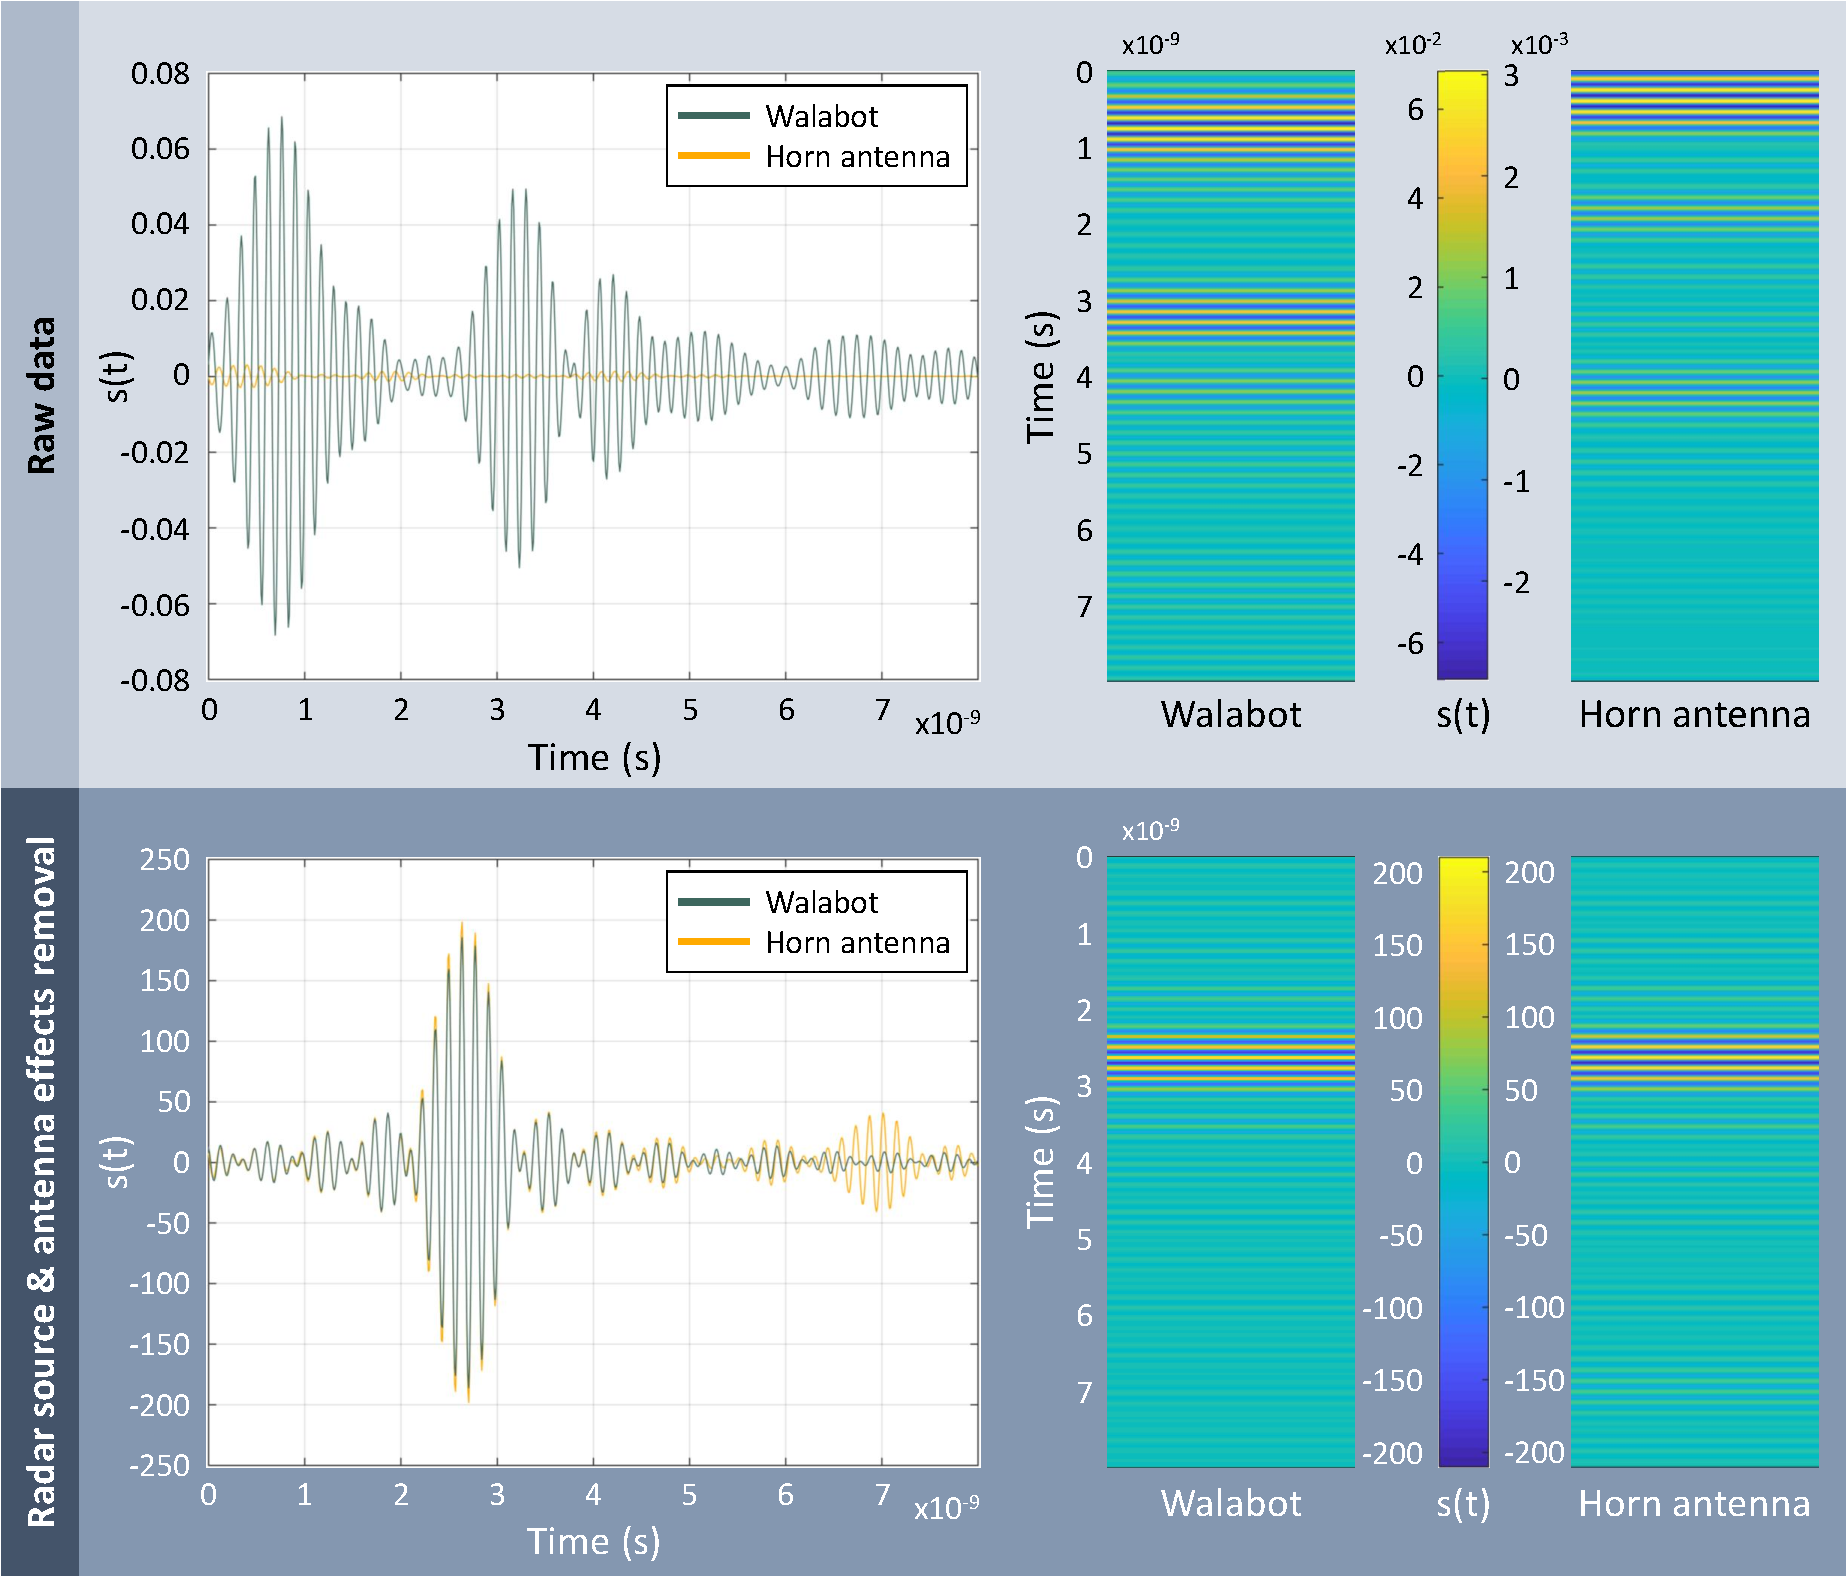
\includegraphics[width=\linewidth]{Figures/RadarChallenges/Pipeline/radar-equivalence.pdf}
    \vspace{-12pt}
    \caption{Radar signal from two radars (Walabot and vector network analyzer + horn antenna) at 40 cm from a large copper plate. The top plots show two representations of the raw time-domain signal. The signals from both radars are at different scales and feature radar source and antenna effects, including internal reflections, making them difficult to compare. The bottom plots show how the signal from both radars is normalized after removing the radar source and antenna effects.}
    \label{fig:radar-challenges:radar-equivalence}
    \vspace{-14pt}
\end{figure*}

%--------------------------------------------------------------------------------%
\subsection{Background Scene Removal} \label{sec:radar-challenges:processing-strategy:background-scene}
Based on the superposition principle, the reflections from static objects in the surrounding environment (\eg walls, plants, furniture) are subtracted from the normalized signal (\fig~\ref{fig:radar-challenges:pipeline}. This leaves only the reflections of moving objects and persons, including the end user, in the resulting signal (property P\textsubscript{2}), resulting in higher accuracy and efficiency of full-wave inversion. It is important to acknowledge that while the interactions between the static objects and the hand are not eliminated with the application of the superposition principle, they are anticipated to be minimal or negligible when the static objects are positioned farther away from the endpoint, as detailed in the following section.
% 
The computational complexity of this stage for processing one radar frame is $O(n)$, where $n$ is the size of the radar signal.

%   Based on the superposition principle, the signal from the surrounding environment (\eg walls, plants, furniture) is subtracted from the normalized signal. The resulting signal only contains the reflections of moving objects and persons, including the user, thus improving the accuracy and efficiency of full-wave inversion.

% A frame of the gesture is subtracted from all the other frames to remove the reflections of static background objects.

%--------------------------------------------------------------------------------%
\subsection{Time Gating} \label{sec:radar-challenges:processing-strategy:time-gating}
An IFFT (Eq.~\ref{eq:radar-challenges:ifft}) is first applied to the signal to convert it to the time domain (\fig~\ref{fig:radar-challenges:pipeline}d), which simplifies subsequent computations.
The time domain signal is then truncated (\fig~\ref{fig:radar-challenges:pipeline}e) to exclude all reflections occurring outside some distance range of the radar (\fig~\ref{fig:radar-challenges:tw} and Eq.~\ref{eq:radar-challenges:tmax}). The distance range is carefully selected to maximize the signal-to-noise ratio while maintaining enough distance between the user and the radar to ensure the validity of our far-field antenna model (Eq.~\ref{eq:radar-challenges:sff6}). Consequently, movements occurring behind the user are ignored, which improves the efficiency of the next stages, and fewer data need to be processed in the full-wave inversion, thus increasing the efficiency of the next stage and enabling faster real-time processing without compromising on accuracy.
%
Because the truncated radar signal is copied into a new frame, the computational complexity of this stage for processing one radar frame is $O(n)$, where $n$ is the size of the truncated radar signal. The computational complexity could be reduced to a constant value ($O(1)$) if the signal was truncated without copying it into a new frame.

% The time domain signal is truncated to keep only reflections within a distance from the radar (see \fig \ref{fig:radar-challenges:tw} and Eq.~\ref{eq:radar-challenges:tmax}). The maximum distance is carefully selected to ensure a sufficient signal-to-noise ratio while maintaining a sufficient distance between the user and the radar. The benefits of this stage are twofold: (1) moving objects behind the user is ignored, thus improving the accuracy of the next stage, and (2) the number of data to process in the full-wave inversion is reduced, thereby increasing the efficiency of the next stage.

%--------------------------------------------------------------------------------%
\subsection{Full-wave Inversion}\label{sec:radar-challenges:processing-strategy:inversion}
The process of full-wave inversion reduces the radar signal to two physically meaningful dimensions (\fig~\ref{fig:radar-challenges:pipeline}e): the hand-radar distance $d$ and the relative permittivity $\epsilon_{r,e}$ of an infinite medium equivalent to the hand. The interface between the air and this medium is situated at a distance $d$ from the radar and is orthogonal to the radar-hand direction. 
The obtained permittivity is an apparent value that remains unaffected by variations in the hand-radar distance. This apparent permittivity is determined by the quantity of signal reflected by the hand and should not be confused with its true permittivity. As such, it provides information on the pose of the hand, whereas the distance gives the dynamic position of the hand.
The inversion algorithm iteratively adjusts the distance and apparent relative permittivity parameters of the model to find the best fit between the modeled and measured signals (Eq.~\ref{eq:radar-challenges:OFTD}). The computations are sped up by the use of a pre-calculated LUT for real-time objective function minimization. 
This drastic data reduction keeps essential information from the radar signal in the form of distance and permittivity values, thus enabling to use of less sophisticated algorithms, such as template-matching algorithms for gesture recognition.
%
The computational complexity of this step is $O(n \cdot k)$, where $n$ is the size of the truncated radar signal and $k$ is the size of the LUT. Despite the use of an LUT, this is the most expensive stage of the pipeline.

We conducted a small experiment to evaluate the sensitivity of the full-wave inversion process to three main variables: (1) the presence of strong reflectors in the background, (2) the distance between the hand and the radar, from 30 cm to 110 cm, and (3) the angle between the hand and the radar, from 0° to 60° at a distance of 30 cm and from 0° to 45° at a distance of 50 cm. 
%
A custom radar (vector network analyzer combined with the BBHA 9120 A horn antenna, 0.8 to 5 GHz, high directivity of 45° 3 dB beamwidth in the E-plane and 30° in the H-plane at 1 GHz) was attached to a 3D positioning system and faced a hollow aluminum box of dimensions 21.6 cm (height) $\times$ 10 cm (width) $\times$ 8 cm (depth) attached to a PVC pole. A 3 m $\times$ 3 m copper plate placed on the wall 127.5 cm behind the aluminum box acted as a strong background reflector. Fig.~\ref{fig:radar-challenges:radar-angle-distance-setup} and~\ref{fig:radar-challenges:radar-angle-distance} illustrate the experimental setup and the results of this experiment. 
%
The copper plate in the background did not have an impact on the inversion process as its reflections were removed in the time gating stage.
%
Similarly, the inversion process correctly estimated the distance between the radar and the aluminum box up to 110 cm. Worse results should be expected when using radars with a lower signal-to-noise ratio and/or estimating the distance of less reflective objects. The maximum interaction distance should thus be adjusted accordingly.
%
The results of the inversion process when increasing the angle between the aluminum box and the radar antenna were consistent with its high directivity of 45°: the inversion process failed to correctly estimate the distance from 40° at 30 cm and 46° at 50 cm.
%
The permittivity estimations changed drastically depending on the distance and angle between the aluminum box and the radar antenna, suggesting that this measure should not be used in scenarios where users are expected to move a lot around the radar. 
Although the electromagnetic model accounts for the decrease of signal strength with respect to distance (3D spherical divergence), these results make sense as the inversion process considers the hand to be an infinite medium to simplify computations. Because the hand is a finite medium, some of the radar signal does not interact with it, resulting in less signal being reflected than anticipated, which corresponds to a lower estimated relative permittivity. This phenomenon is emphasized when the hand is moved further away and/or more offset from the radar antenna. 
%
We believe that the model could be improved to account for the finite size of the hand, thus providing an estimation of relative permittivity that would be independent of the hand-radar distance.

\begin{figure}
    \centering
    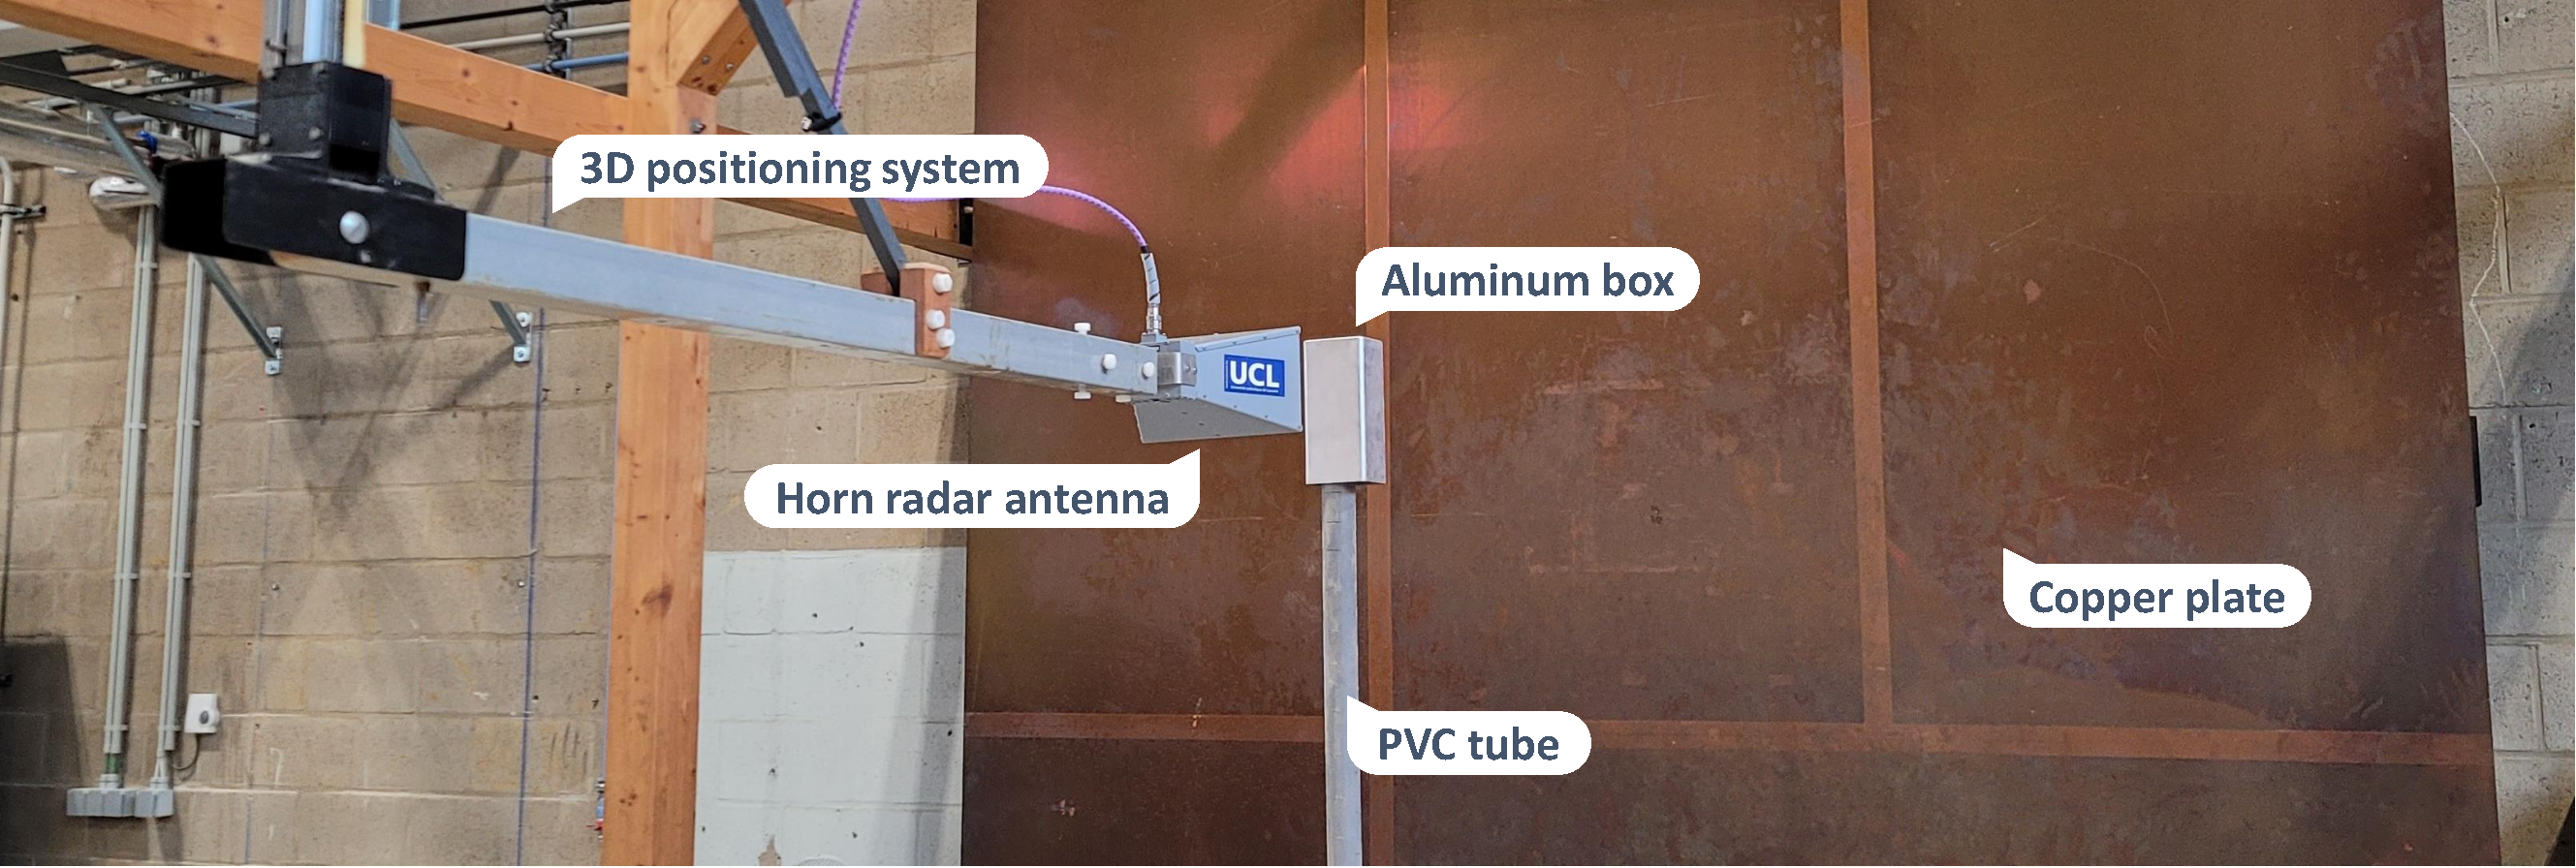
\includegraphics[width=\linewidth]{Figures/RadarChallenges/Pipeline/horn-experimental-setup.pdf}
    \vspace{-12pt}
    \caption{Experimental setup for evaluating the sensitivity of the full-wave inversion process with respect to distance, angle, and background scene.}
    \label{fig:radar-challenges:radar-angle-distance-setup}
    \vspace{-14pt}
\end{figure}


\begin{figure*}
    \centering
    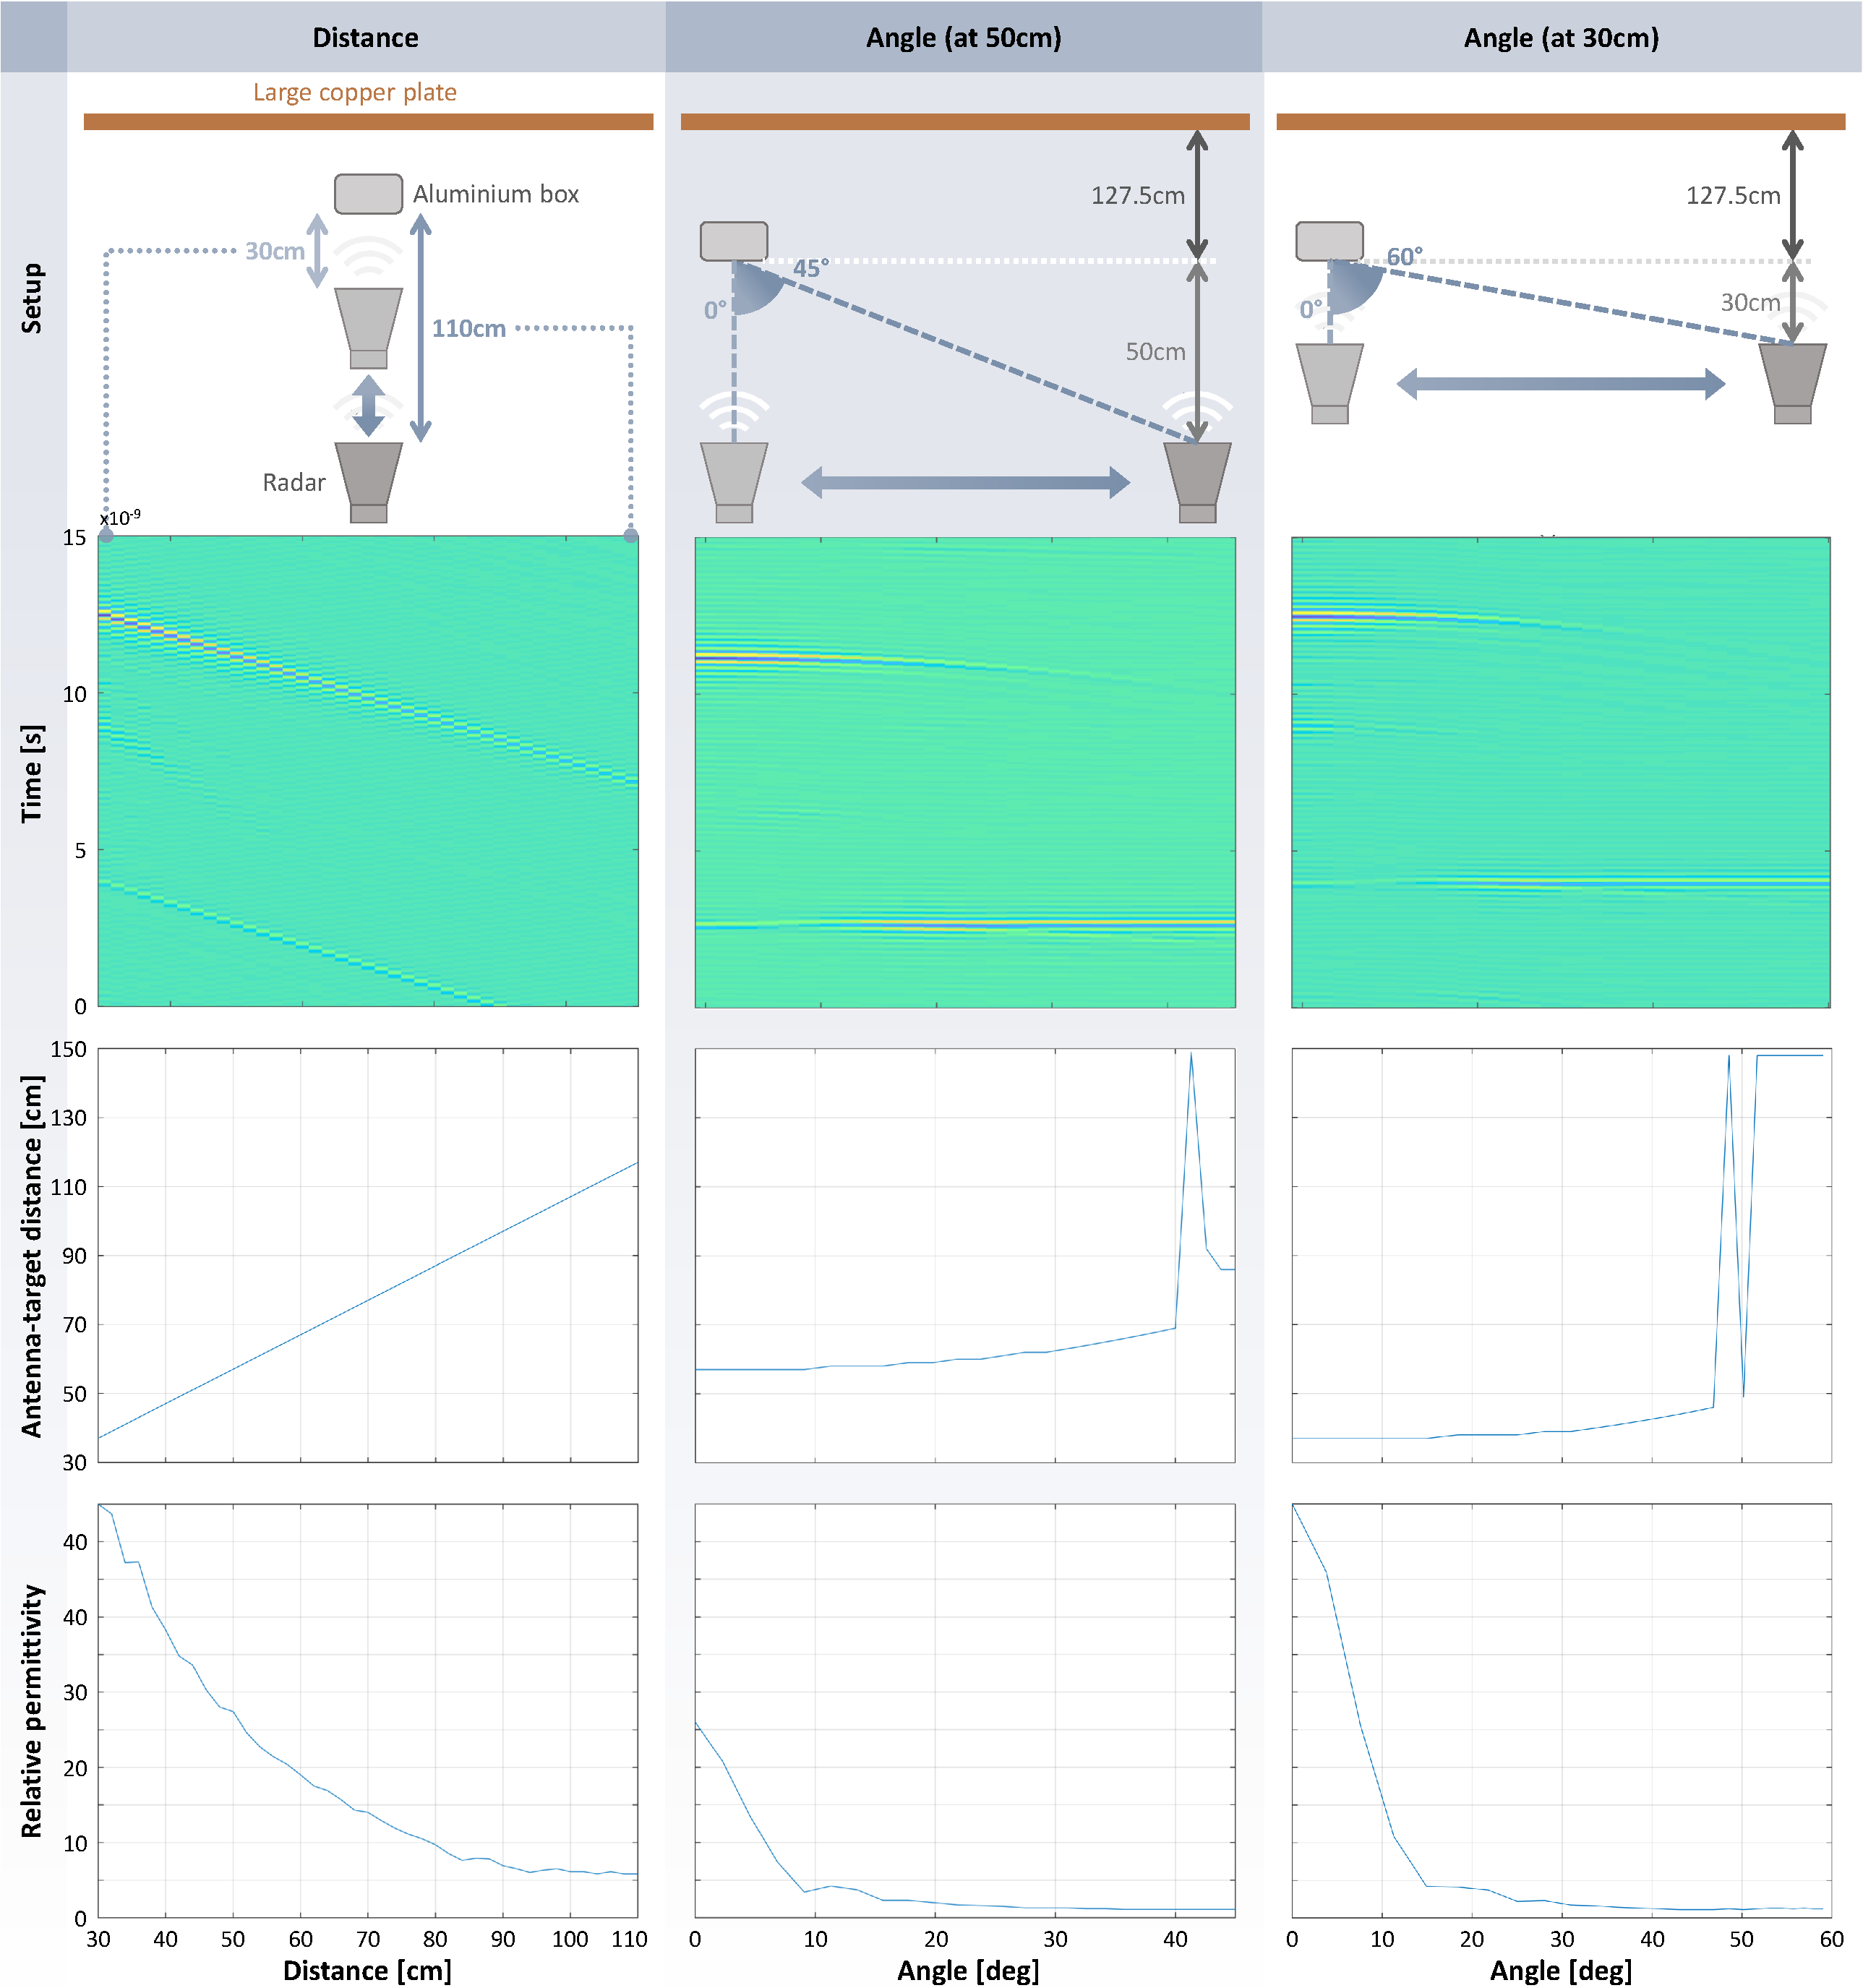
\includegraphics[width=\linewidth]{Figures/RadarChallenges/Pipeline/effect-of-angle-distance.pdf}
    \vspace{-12pt}
    \caption{Effect of radar-target angle and distance on the signal after radar source and antenna effects removal and after inversion.}
    \label{fig:radar-challenges:radar-angle-distance}
    \vspace{-14pt}
\end{figure*}

% The radar signal is reduced to two physically meaningful dimensions by the process of full-wave inversion, namely the hand-radar distance and the relative permittivity of an infinite plane equivalent to the hand. Therefore, the retrieved permittivity is an apparent permittivity and not the true permittivity of the hand. Distance gives an idea of the position of the hand, whereas apparent permittivity provides information on the pose of the hand.
% The inversion process consists of adjusting the distance and apparent relative permittivity parameters of a model to find the best fit between the modeled and measured signals (Eq.~\ref{eq:radar-challenges:OFTD}). This process is sped up by the use of a pre-calculated LUT. The drastic data reduction, while keeping essential information, resulting from the full-wave inversion enables the use of simple template matching algorithms for gesture recognition.



% Extract two physically relevant features from the time-domain radar signal: permittivity and distance. The former represents the distance between the user's hand and the radar, while the latter is the effective permittivity of the infinite plane defined by the surface of the hand and gives insights into the configuration of the hand (\eg its orientation with respect to the radar).


%--------------------------------------------------------------------------------%
\subsection{Filtering} \label{sec:radar-challenges:processing-strategy:filtering}
The result of the full-wave inversion depends on the signal-to-noise ratio, \ie on the quality of the radar data. 
A low signal-to-noise ratio and moving objects behind or in front of the user may produce an incorrect estimation of the distance and apparent permittivity. Two strategies are employed to clean up the signal produced by the inversion stage (\fig~\ref{fig:radar-challenges:pipeline}f). First, the distance and permittivity values are discarded and replaced with default values ($d{=}75 cm$, $\epsilon_{r,e}{=}1.0$) when the estimated permittivity is close to the relative permittivity of the air, \ie when no hand is detected in front of the radar. In addition, a moving median filter is applied to smooth out too-fast variations in the estimated distance and permittivity. The moving median filter was selected for its ability to filter out large and sudden variations in the data that would not be physically possible.
Employing radars with a large dynamic range and leading to a higher signal-to-noise ratio and a wider field of view could decrease the need for filtering, as they would better dissociate the hand signal from the noise and hand reflections, even when the hand is not perfectly in front of the radar.
%
The computational complexity of this stage for processing one radar frame is constant ($O(1)$) as the signal after inversion from one receiving antenna is always reduced to 2 dimensions regardless of its initial size.

% %================================================================================%
\section{Implementation} \label{sec:radar-challenges:implementation}
The radar data processing strategy was initially implemented based on MATLAB scripts provided by Prof. Sébastien Lambot that were adapted to automatically process an entire gesture dataset. However, these scripts were slow and could not be adapted easily for real-time gesture recognition.
%
Prof. Sébastien Lambot and his team later converted parts of the MATLAB scripts to C++, which we assembled and optimized for real-time gesture recognition and faster batch processing of gestures.
Both the MATLAB and C++ versions of the batch processing pipeline compile all processed gestures into the \ql dataset format. 
The C++ real-time version of the pipeline initializes a WebSocket server through which it can send processed radar data to other applications, such as the \ql framework (Chapter~\ref{chap:quantumleap}).

\begin{figure}[t]
\centering
\begin{subfigure}{.49\textwidth}
    \centering
    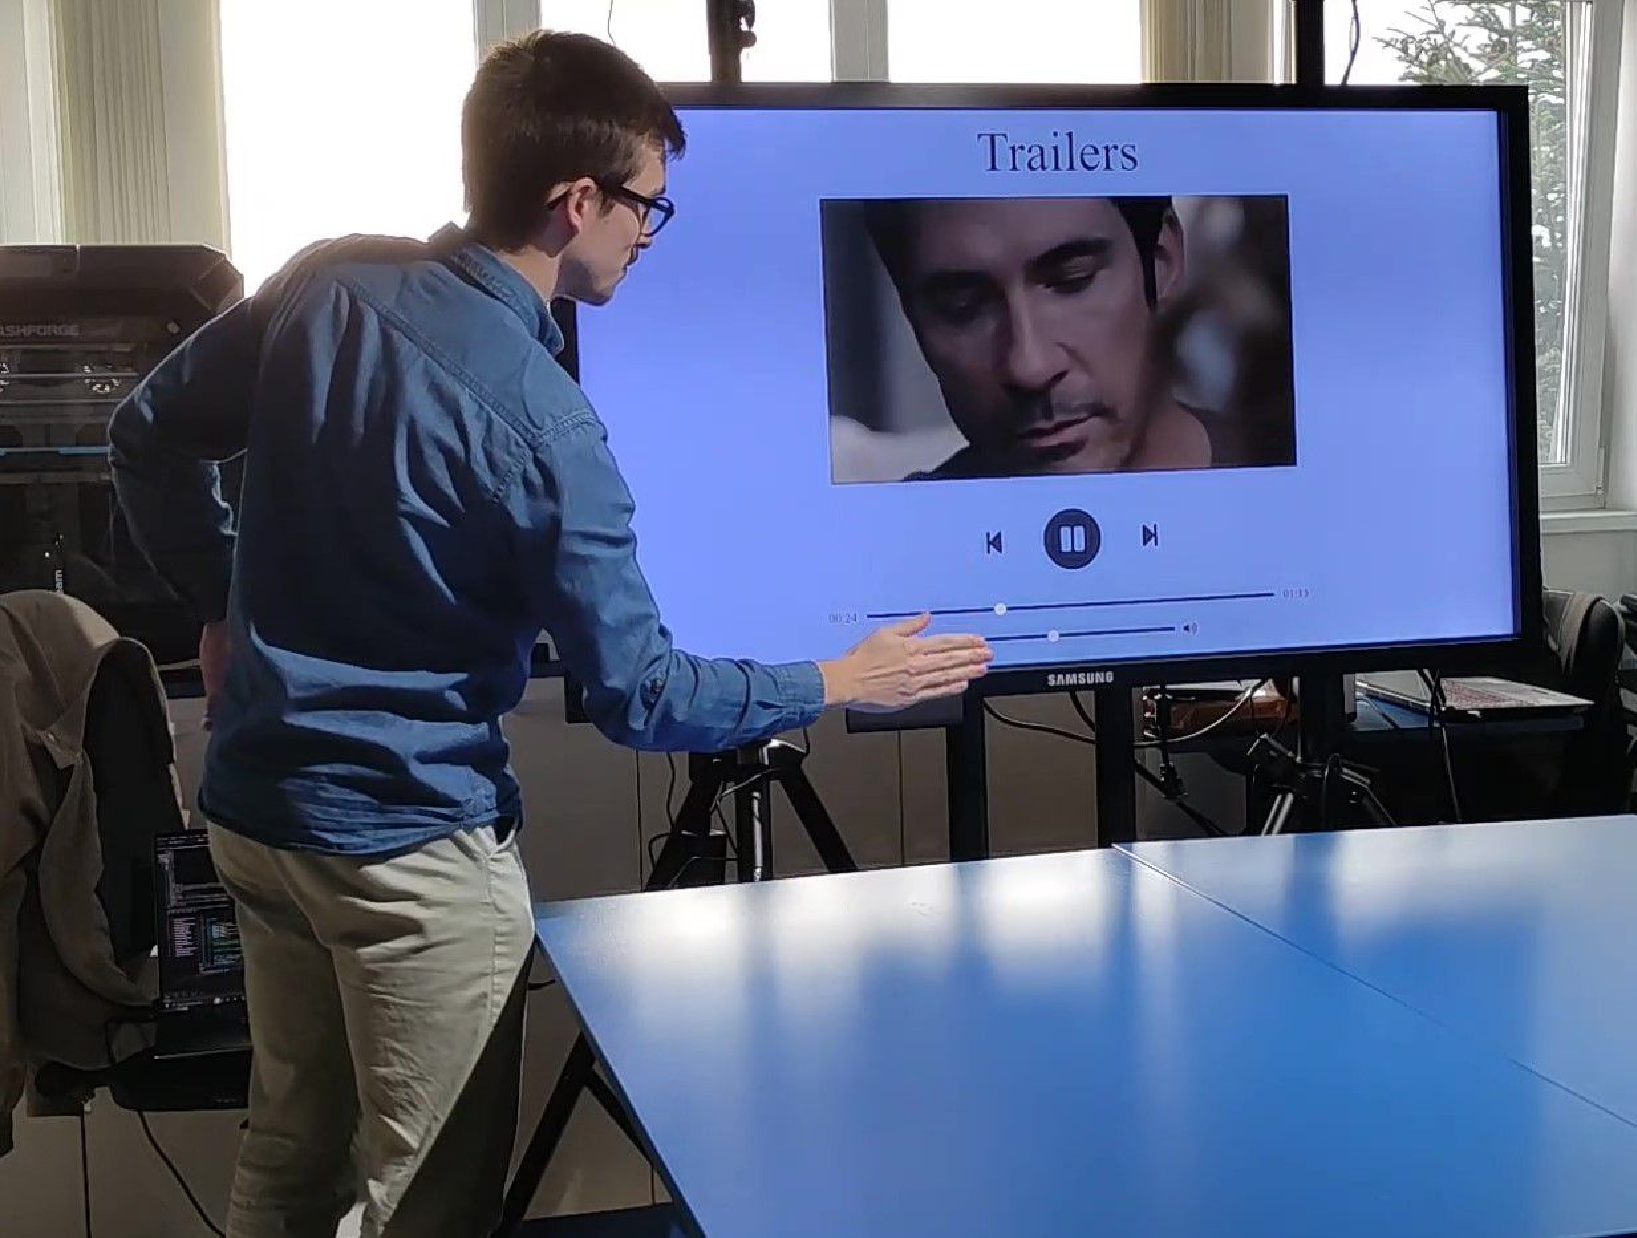
\includegraphics[width=\linewidth]{Figures/RadarChallenges/Application/app-screen-2.pdf}  
    \vspace{-15pt}
    \captionsetup{width=.9\linewidth}
    \caption{Radar placed on the screen.}
    \label{fig:radar-challenges:screen}
\end{subfigure}
\begin{subfigure}{.49\textwidth}
    \centering
    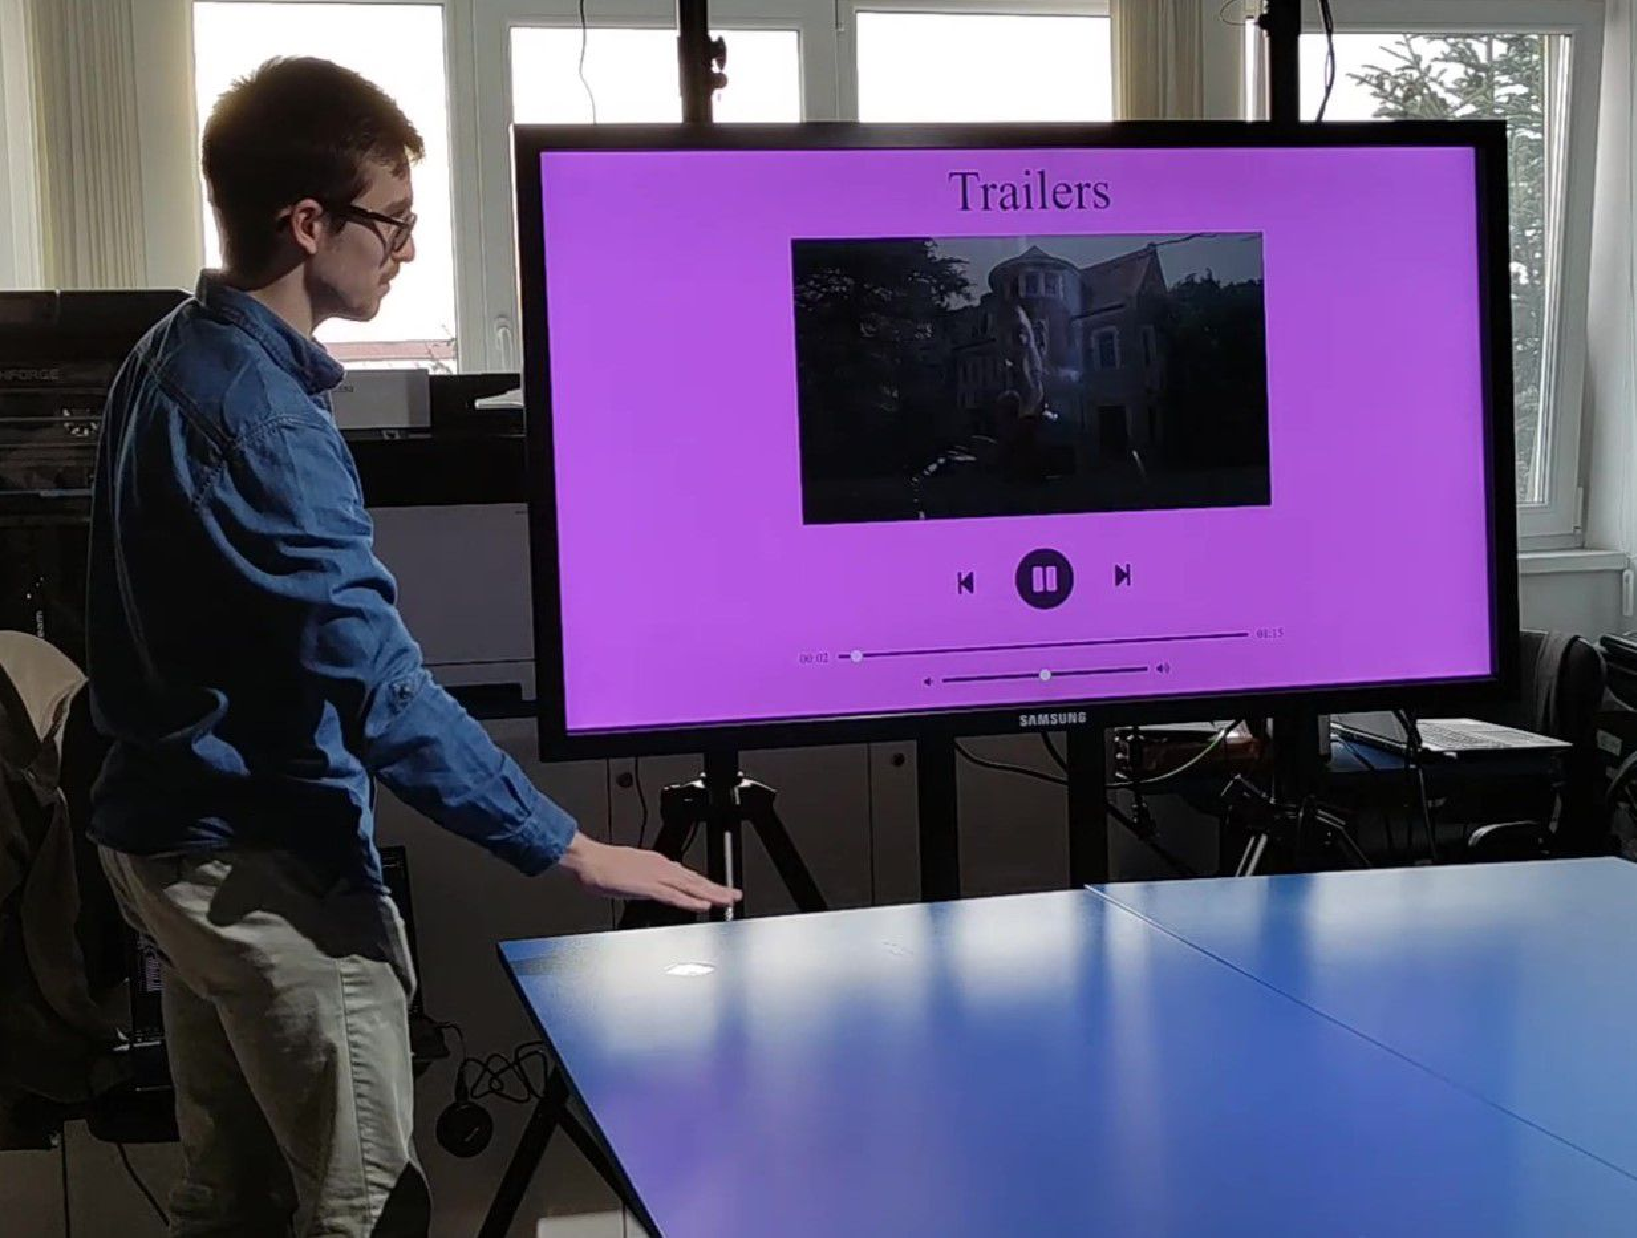
\includegraphics[width=\linewidth]{Figures/RadarChallenges/Application/app-table-2.pdf}  
    \vspace{-15pt}
    \captionsetup{width=.9\linewidth}
    \caption{Radar placed under the table.}
    \label{fig:radar-challenges:application:table}
\end{subfigure}
\vspace{-8pt}
\caption{Screenshots of the prototype application in two configurations.}
\label{fig:radar-challenges:application}
% \vspace{-12pt}
\end{figure}

This version of the pipeline was used in a simple prototype application as part of the RadarSense project in Suceava, Romania, which combined touch- and radar-based gestures for manipulating videos on a large screen (\fig~\ref{fig:radar-challenges:application}). Users could interact with videos using touch gestures and switch between categories by pushing their palm towards a radar placed under the table or attached to the screen.

% %================================================================================%
\section{Limitations} \label{sec:radar-challenges:limitations}
This section discusses the main limitations of our approach.
%
First, our pipeline does not take into account variations in position with respect to the radar, as shown in Section~\ref{sec:radar-challenges:inversion} and \fig~\ref{fig:radar-challenges:radar-angle-distance}, resulting in inaccurate permittivity estimations that change drastically depending on the distance and angle between the user and the radar.
%
Second, our signal processing pipeline neglects anatomical differences between users (\eg hand size, arm length), which may lower the effectiveness of gesture recognition algorithms in user-independent scenarios (Section~\ref{sec:quantumleap-testing:description:testing-procedures:user-scenarios}). For example, a larger hand will reflect more signal back towards the radar, resulting in a greater relative permittivity measured for the same gesture. Taking into account these variations would require at least three changes to the pipeline: (1) normalize the amplitude of user reflections with respect to their hand and body size, (2) extract the hand-body distance instead of the hand-radar distance in the inversion stage, and (3) normalize the hand-body distance with respect to the user's arm length.

% processing + real-time
% matlab and C++ for batch processing
% C++ for real-time processing

% The pipeline was used in a simple application in the RadarSense project(from Romania)

% %================================================================================%
% \section{Gesture Sets}

%================================================================================%
\section{Conclusion} \label{sec:radar-challenges:conclusion}
% Summary
The use of microwave radar sensors for gesture recognition has several advantages compared to vision-based sensors, including less sensitivity to environmental conditions. However, because of the complexity of radar signals, most of the existing work on this topic has relied on complex machine-learning approaches.
%
In this chapter, we introduced a full-wave electromagnetic model and inversion-based approach for radar signal processing, which removes radar source and antenna effects from raw radar signals, eliminates the reflections of static objects in the vicinity of the radar and moving objects behind the user, and reduces these signals to two physically meaningful features, the hand-radar distance and the effective permittivity of the hand.
%
Two small experiments were conducted to investigate the efficacy of our pipeline.
The first experiment showed that the pipeline could effectively normalize signals from two distinct radars, including a Walabot and a custom radar equipped with a horn antenna.
The second investigated the sensitivity of our pipeline to variations in radar-target distance and angle and showed that signals from our processing pipeline changed with both radar-target distance and angle.    
% Implementation
Multiple versions of the pipeline were implemented in MATLAB and C++ for batch and real-time signal processing, and a prototype application was created to showcase the system. 

% Software quality properties
This chapter addresses the four software quality properties outlined in Section~\ref{sec:introduction:research:research-questions}.
%
Regarding \textit{compatibility}, our pipeline introduces a degree of interoperability between radar systems by normalizing their signals. Datasets produced with one radar could thus be reused with another one, provided they operate at comparable frequency ranges. This interoperability was illustrated in Section~\ref{sec:radar-challenges:antenna-effects}, which compared the normalized signals from two different radar systems.
%
Similarly, this normalization of radar signals contributes to \textit{maintainability} and \textit{portability}. For instance, a radar and its corresponding gesture set can be used in a new environment without having to re-record all of the gestures, requiring only a new snapshot of the background scene. Similarly, the pipeline can accommodate new radar systems after they have been properly calibrated. 
%
In terms of \textit{usability}, the normalization applied by our pipeline could improve gesture recognition accuracy, thus resulting in more usable gestural interfaces. 

% Future works
We identify three main avenues for future research. 
%
First, the pipeline could be modified to take into account two elements: the finite size of the hand, to provide an estimation of relative permittivity independent of the hand-radar distance, and anatomical differences between users.
%
Future work could also explore the possibility of employing trilateration with data from the full-wave inversion stage produced by a set of spatially separated antennas to compute a 3D position of the hand. This would have multiple benefits, including being able to display a cursor on the screen and enabling more accurate recognition of 3D hand trajectories.
%
Finally, we could look into implementing techniques for gesture segmentation to facilitate complex real-time gesture interaction.